% Author: Izaak Neutelings (December 2022)
% Sources:
%   https://arxiv.org/abs/2201.08458
%   https://cms-results.web.cern.ch/cms-results/public-results/publications/TAU-20-001/index.html
\documentclass[border=3pt,tikz]{standalone}
\usepackage{amsmath,amssymb}
\usepackage{bm} % math bold
\usepackage{tikz}
\usetikzlibrary{patterns}
\usepackage[outline]{contour} % glow around text
\contourlength{1.2pt}
\tikzset{>=latex}

\colorlet{myred}{red!90!black}
\colorlet{myblue}{blue!80!black}
\colorlet{mydarkred}{red!40!black}
\colorlet{mydarkblue}{blue!40!black}
\tikzstyle{mythin}=[line width=0.3pt]
\tikzstyle{mythick}=[line width=0.6pt]
\tikzstyle{mydouble}=[white,double=#1,double distance=0.4pt,line width=0.3pt]
\tikzstyle{axis}=[->,mythick]
%\def\tick[#1](#2){\draw[thick] (#2) ++ (#1:#3/2) --++ (#1-180:#3)}
\def\tick[#1:#2](#3){\draw[mythick] (#3) ++ (#1:#2/2) --++ (#1-180:#2)}
\newcommand{\tauh}{\tau_\mathrm{h}}

\begin{document}


% DEEPTAU INPUT GRID for convolutional layers
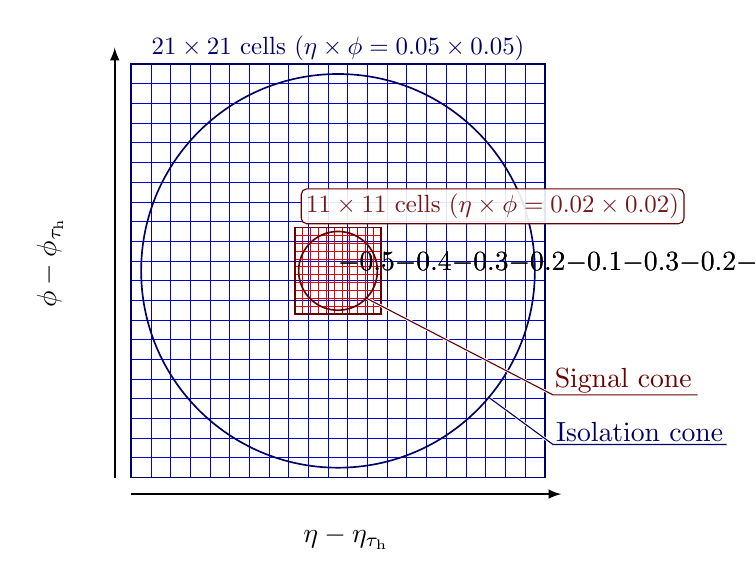
\begin{tikzpicture}[scale=5]
  \def\n{11} % number of cells in inner grid
  \def\N{21} % number of cells in outer grid
  \def\a{0.02} % cell size in inner grid
  \def\A{0.05} % cell size in inner grid
  %\def\w{0.22} % total inner width W = 11*0.02 = 0.22
  %\def\W{1.05} % total outer width W = 21*0.05 = 1.05
  \pgfmathsetmacro\w{\n*\a} % total inner width W = 11*0.02 = 0.22
  \pgfmathsetmacro\W{\N*\A} % total outer width W = 21*0.05 = 1.05
  \def\r{0.10} % radius of signal cone
  \def\R{0.50} % radius of isolation cone
  
  % GRIDS
  %\def\mygrid[#1]#2#3{
  %  \draw[#1,shift={(-#3/2,-#3/2)}] (0,0) grid[step=#2] (#3,#3);
  %  \draw[#1,black] (-#3/2,-#3/2) rectangle++ (#3,#3);
  %}
  \draw[myblue,mythin,shift={(-\W/2,-\W/2)}] (0,0) grid[step=\A] (\W,\W);
  \draw[myred, mythin,shift={(-\w/2,-\w/2)}] (0,0) grid[step=\a] (\w,\w);
  \draw[mydarkblue,mythick] (-\W/2,-\W/2) rectangle++ (\W,\W);
  \draw[mydarkred,mythick] (-\w/2,-\w/2) rectangle++ (\w,\w);
  
  % SIGNAL & ISOLATION CONES
  \draw[mydouble=mydarkblue] (-40:\R) -- (0.52*\W,-0.42*\W)
    node[mydarkblue,above right=0pt,inner sep=1pt] (IC) {Isolation cone}
    --++ (0.42*\W,0); %(IC.south east);
  \draw[mydarkblue,line width=0.6] (0,0) circle(\R);
  \draw[mydouble=mydarkred] (-44:\r) -- (0.52*\W,-0.30*\W)
    node[mydarkred,above right=-0.5pt,inner sep=1pt] (SC) {Signal cone}
    --++ (0.35*\W,0); %(SC.south east);
  \draw[mydarkred,line width=0.6] (0,0) circle(\r);
  
  % CELL LABELS
  \node[mydarkblue,above=-2pt,scale=0.9] at (0,\W/2)
    {$\N\times\N$ cells ($\eta\times\phi=\A\times\A$)};
  \node[mydarkred,draw,rounded corners=2pt,fill=white,fill opacity=0.9,
        above=-1pt,align=left,above right,inner sep=2pt,scale=0.9] at (-0.43*\w,0.57*\w)
    {$\n\times\n$ cells %\\
     ($\eta\times\phi=\a\times\a$)};
  
  % X AXIS
  \pgfkeys{/pgf/number format/.cd,fixed,precision=1} % rounding errors
  \begin{scope}[shift={(0,-0.54*\W)}]
    \draw[axis] (-\W/2,0) --++ (1.04*\W,0)
      node[midway,below=8pt] {$\eta-\eta_{\tauh}$};
    \foreach \x in {-0.5,-0.4,...,0,...,0.501}{ % major ticks
      \tick[90:0.03](\x,0) node[below,scale=0.6] {$\pgfmathprintnumber{\x}$};
    }
    \foreach \x in {-0.45,-0.35,...,0,...,0.451}{ % minor ticks
      \tick[90:0.02](\x,0);
    }
  \end{scope}
  
  % Y AXIS
  \begin{scope}[shift={(-0.54*\W,0)}]
    \draw[axis] (0,-\W/2) --++ (0,1.04*\W)
      node[midway,rotate=90,above=15pt] {$\phi-\phi_{\tauh}$};
    \foreach \y in {-0.5,-0.4,...,0,...,0.501}{ % major ticks
      \tick[0:0.03](0,\y) node[left=-0.8pt,scale=0.6] {$\pgfmathprintnumber{\y}$};
    }
    \foreach \y in {-0.45,-0.35,...,0,...,0.451}{ % minor ticks
      \tick[0:0.02](0,\y);
    }
  \end{scope}
  
  
\end{tikzpicture}


\end{document}
